
\section{Methodology}



The SleepGCN-Transformer is a hybrid deep learning framework designed for accurate sleep stage classification by combining the strengths of Graph Convolutional Networks (GCNs) and Transformer architectures. This model is trained on the Sleep-EDF dataset, utilizing four critical physiological signal channels: EEG Fpz-Cz, EEG Pz-Oz, EOG (horizontal), and submental EMG.

In this architecture, GCNs are employed to capture spatial relationships between the multimodal input signals, while the Transformer encoder is tasked with modeling the temporal dependencies across time sequences. This dual approach ensures that both spatial and sequential dynamics are effectively learned.

Experimental results confirm the effectiveness of the model, achieving an accuracy of 93.12\% on the training set and 93.04\% on the validation set. To address class imbalance—particularly the underrepresentation of certain sleep stages—the model incorporates Focal Loss, which emphasizes harder-to-classify samples during training.

Further analysis of feature importance revealed that the EMG and EEG Pz-Oz channels play a significant role in predicting sleep stages. This methodological framework not only enhances classification performance but also supports the integration of explainable AI techniques, contributing to the development of interpretable tools for clinical sleep analysis and decision-making.

\begin{figure}
	\centering
	\includegraphics[width=.9\linewidth]{"img/paper_3/Graph Convolution Neural Network -SleepGCN_Transformer Architechture"}
	\caption{Proposed Architecture of the sleep GCN- Transformer Architecture}
	\label{fig:graph-convolution-neural-network--sleepgcntransformer-architechture}
\end{figure}


\section{Dataset and Implementation Environment}

Our experiments were conducted using the publicly available Sleep-EDF dataset, which is widely utilized for sleep stage classification research. The dataset can be accessed at \url{https://physionet.org/content/sleep-edfx/1.0.0/}, and it includes EEG recordings labeled with corresponding sleep stages, enabling effective supervised learning.

The implementation was carried out in Python 3.13.1 using the PyTorch deep learning framework. Development was performed in Visual Studio Code (VS Code) on a machine powered by the Apple M1 chip, utilizing both CPU and Metal acceleration capabilities for training efficiency.

For version control and collaborative development, we used GitHub to manage our codebase. The repository containing our source code is publicly available at \url{https://github.com/tanmay007thor/GCN}.

The source code of this research is licensed under the Apache License 2.0, which allows for open use and distribution. The license details are available at \url{http://www.apache.org/licenses/}.

To support data processing, model training, and evaluation, we relied on several key Python libraries. The primary libraries and their versions used in our project include: NumPy 2.2.2, Pandas 2.2.3, Scikit-learn 1.6.1, SciPy 1.15.1, Matplotlib 3.10.0, Seaborn 0.13.2, PyTorch 2.6.0, Torch Geometric 2.6.1, NetworkX 3.4.2, and MNE 1.9.0. This software environment ensured a reliable, efficient, and reproducible workflow throughout our research.




\section{Preprocessing Techniques}
\begin{figure}[H]
	\centering
	\begin{minipage}{0.48\textwidth}
		\centering
		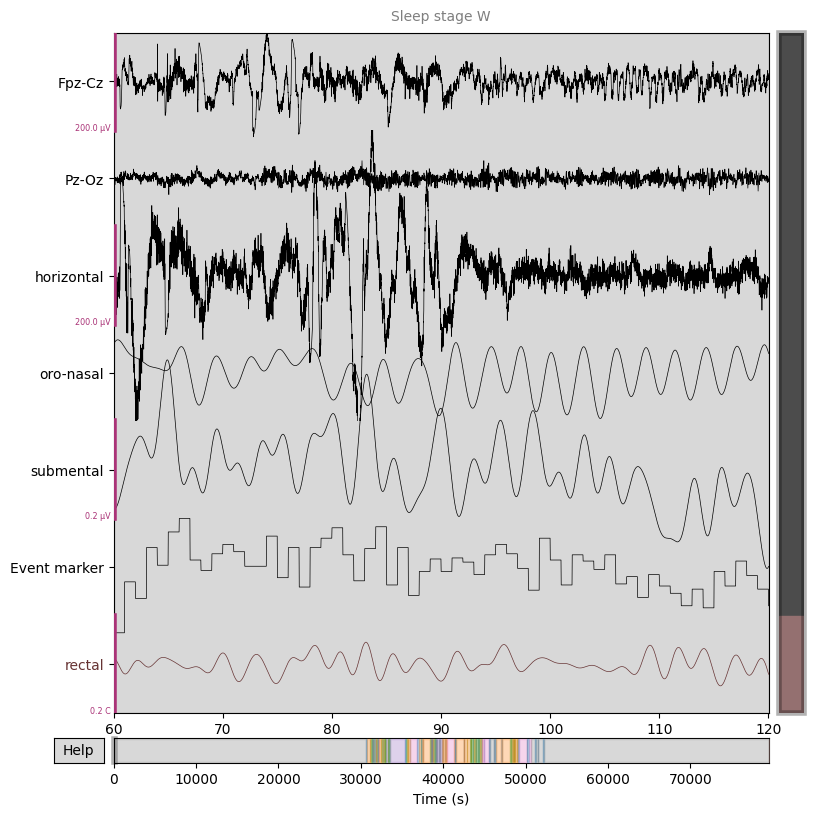
\includegraphics[width=\linewidth]{img/paper_3/Signals}
		\caption{Raw signal channels from the Sleep-EDF dataset}
		\label{fig:raw_signals}
	\end{minipage}
	\hfill
	\begin{minipage}{0.48\textwidth}
		\centering
		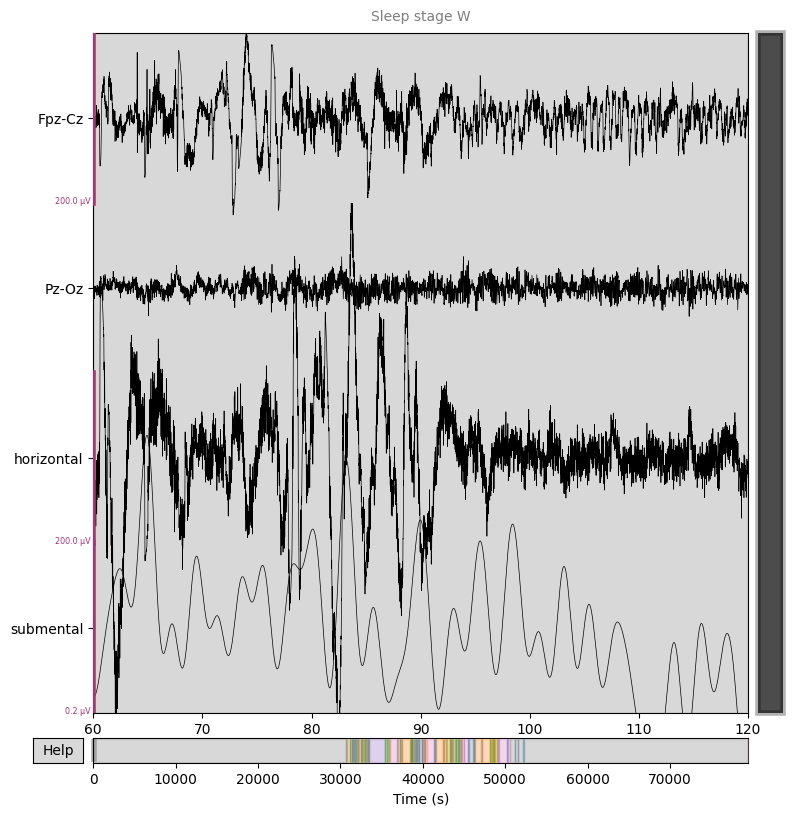
\includegraphics[width=\linewidth]{img/paper_3/filtered chanels}
		\caption{Preprocessed and filtered signal channels}
		\label{fig:filtered_signals}
	\end{minipage}
\end{figure}


\subsection{Data Information}

The Sleep-EDF dataset comprises multichannel physiological signals, including EEG, EOG, EMG, nasal airflow, and temperature, each accompanied by event markers. These signals are recorded over 60-second intervals, with frequency content varying between 60 and 120 Hz. The dynamic nature of these signals introduces significant variability, making it challenging to identify consistent patterns for classification. Such rapid fluctuations can increase the likelihood of misclassification. Furthermore, the dataset presents several challenges such as high-frequency noise, class imbalance (notably a dominance of the Wake stage), and a substantial number of time steps—approximately 100 time steps per second—adding complexity to the task of modeling sleep stages.

\subsection{Preprocessing Pipeline}

To address these challenges, we developed a comprehensive preprocessing pipeline focused on selecting the most informative channels and reducing irrelevant data. Initially, we discarded several channels that were found to contribute minimally to sleep stage classification. The retained signals included the EEG channels (Fpz-Cz and Pz-Oz), the horizontal EOG channel (to track eye movement), and the submental EMG channel (for monitoring chin muscle activity).

Each sleep stage in the dataset was mapped to a simplified class label to consolidate similar stages and reduce classification ambiguity. Table~\ref{tab:sleep_stage_mapping} presents the sleep stage-to-class mapping:

\begin{table}[H]
	\centering
	\caption{Sleep Stage Mapping}
	\label{tab:sleep_stage_mapping}
	\begin{tabular}{llc}
		\hline
		\textbf{Sleep Stage} & \textbf{Label} & \textbf{Mapped Class} \\
		\hline
		Wake                & 0 & 0 \\
		Stage 1             & 1 & 1 \\
		Stage 2             & 2 & 2 \\
		Stage 3             & 3 & 3 \\
		Stage 4             & 4 & 3 \\
		REM                 & 5 & 4 \\
		\hline
	\end{tabular}
\end{table}

The preprocessing begins with reading the EDF recordings and assigning sleep labels based on the mapped classes. Subsequently, we applied a bandpass filter to isolate relevant frequency ranges. Specifically, the signal was filtered to retain only the 0.3–30 Hz band using the `firwin` filter design, effectively removing noise and irrelevant frequencies outside this band. Though not a standard approach, this customized filtering was found to be better suited to our specific dataset and classification task.

We then segmented the signals into fixed-length epochs of 30 seconds. The final preprocessed data was shaped into a three-dimensional format: $(X, 4, 3000)$, where $X$ is the number of epochs (samples), $4$ is the number of selected channels, and $3000$ corresponds to the number of time steps per epoch.

\subsection{Filtering Method}

The filtering was implemented using a windowed time-domain design via the `firwin` method. A Hamming window was employed, configured with a 0.0194 passband ripple and 53 dB stopband attenuation. The filter characteristics were as follows: lower passband edge at 0.30 Hz, lower transition bandwidth of 0.30 Hz (with a $-6$ dB cutoff at 0.15 Hz), upper passband edge at 30.00 Hz, and an upper transition bandwidth of 7.50 Hz (with a $-6$ dB cutoff at 33.75 Hz). These settings were carefully chosen to preserve the signal components relevant to sleep staging while minimizing noise.





\section{Model Architecture and Learning Framework}

To extract spatial features from the multi-channel data, we construct a graph using the four selected channels, where each channel acts as a node and the edges represent their interrelationships. These edges are weighted based on prior literature and empirical observations, assigning higher importance to EEG channels due to their strong influence on sleep stage detection. In contrast, connections involving EMG and EOG are assigned lower weights, as EOG shows weaker correlations. Although assigning self-loop weights is possible, we chose not to include them in this implementation.

The final dataset comprises 11,076 samples, structured as \texttt{Data(x=[3000, 4], edge\_index=[2, 12], edge\_attr=[12], y=[1])}. Here, \texttt{x} represents the time-series data with 3,000 time steps across 4 channels, \texttt{edge\_index} defines the graph connectivity, \texttt{edge\_attr} contains the edge weights, and \texttt{y} denotes the sleep stage label. This dataset is created using the \texttt{SleepEEGDataset} class and is designed to effectively model spatial dependencies across EEG, EMG, and EOG signals, thereby enhancing sleep stage classification performance.


\begin{figure}
	\centering
	\includegraphics[width=0.7\linewidth]{"img/paper_3/Graph Weightage"}
	\caption{Graph Dataset Creation}
	\label{fig:graph-weightage}
\end{figure}

\subsection{GCN Architecture}

To capture spatial dependencies across the selected EEG, EMG, and EOG channels, we incorporate a Graph Convolutional Network (GCN) into our model. Each sample is structured as a graph with four nodes—corresponding to the four selected channels—and each node contains a time series of 3,000 time steps. The dataset comprises 11,076 such graph-based samples.

The GCN consists of five identical graph convolution layers. The initial input has a shape of (4, 3000), which is projected to (4, 256) after the first graph convolution. Each layer includes batch normalization (256 units), followed by a ReLU activation function and a dropout of 0.1. After the final GCN layer, we apply global mean pooling to obtain a graph-level representation.

The propagation rule used in each GCN layer is given by:

\begin{equation}
	H^{(l+1)} = \sigma\left(\tilde{D}^{-1/2} \tilde{A} \tilde{D}^{-1/2} H^{(l)} W^{(l)}\right)
\end{equation}

\begin{itemize}
	\item $H^{(l)} \in \mathbb{R}^{N \times D}$ is the feature matrix at layer $l$, where $N$ is the number of nodes and $D$ is the feature dimension.
	\item $\tilde{A} = A + I$ is the adjacency matrix with self-loops.
	\item $\tilde{D}$ is the degree matrix corresponding to $\tilde{A}$.
	\item $W^{(l)}$ is the learnable weight matrix for layer $l$.
	\item $\sigma$ denotes a non-linear activation function, typically ReLU.
\end{itemize}

The simplified form for one GCN layer operation is:

\begin{equation}
	X' = \sigma\left(\tilde{D}^{-1/2} \tilde{A} \tilde{D}^{-1/2} X W\right)
\end{equation}

To aggregate node features into a graph-level embedding, we use global mean pooling:

\begin{equation}
	x = \frac{1}{|V|} \sum_{v \in V} h_v
\end{equation}

\begin{itemize}
	\item $V$ is the set of nodes in the graph.
	\item $h_v$ is the feature vector of node $v$.
	\item $x$ is the pooled feature vector representing the entire graph.
\end{itemize}

We apply standard activation and normalization functions during training:

\begin{equation}
	\text{ReLU}(x) = \max(0, x)
\end{equation}

\begin{equation}
	\text{softmax}(x_i) = \frac{e^{x_i}}{\sum_j e^{x_j}}
\end{equation}

\begin{equation}
	x'' = \frac{x' - \mu}{\sigma}
\end{equation}

\begin{itemize}
	\item $\mu$ is the mean of $x'$.
	\item $\sigma$ is the standard deviation of $x'$.
	\item $x''$ is the normalized feature representation.
\end{itemize}


\subsection{Transformer Architecture}

To capture temporal dependencies in the input signal, we utilize a Transformer encoder comprising two stacked layers. Initially, the input is projected into a continuous vector space using an embedding layer. Since Transformers lack inherent mechanisms for handling sequential order, positional encodings are added to preserve time-step information. 

Following embedding and encoding, we use multi-head self-attention to allow the model to focus on different aspects of the signal simultaneously. The attention outputs are concatenated and passed through a feedforward network with dropout regularization. Finally, a fully connected classifier outputs logits for four-class sleep stage classification.

The operations within the Transformer encoder are summarized using the following equations:
\subsection{Transformer: Key Components and Equations}

\begin{itemize}
	\item \textbf{Input Embedding:} Maps input tokens into a continuous vector space.
	\begin{equation}
		X_{\text{embed}} = X W_{\text{embed}}
	\end{equation}
	
	\item \textbf{Positional Encoding:} Adds sequence order information using sine and cosine functions.
	\begin{equation}
		PE(\text{pos}, 2i) = \sin\left(\frac{\text{pos}}{10000^{2i/d}}\right)
	\end{equation}
	\begin{equation}
		PE(\text{pos}, 2i+1) = \cos\left(\frac{\text{pos}}{10000^{2i/d}}\right)
	\end{equation}
	
	\item \textbf{Query, Key, and Value Computation:} Core of attention mechanism, derived from input.
	\begin{equation}
		Q = XW_q,\quad K = XW_k,\quad V = XW_v
	\end{equation}
	
	\item \textbf{Scaled Dot-Product Attention:} Computes weighted output of values using attention scores.
	\begin{equation}
		H_1 = \text{softmax}\left(\frac{QK^T}{\sqrt{d_k}}\right) V
	\end{equation}
	
	\item \textbf{Multi-Head Attention:} Combines multiple attention outputs for diverse feature learning.
	\begin{equation}
		H = \text{Concat}(H_1, H_2, ..., H_h) W_0
	\end{equation}
\end{itemize}














\subsection{Training Pipeline}

The training process for the SleepGCN-Transformer model is designed to handle class imbalance, prevent overfitting, and improve generalization. Below, we outline the training methodology using key equations:

\textbf{Label Smoothing:} To reduce overconfidence in predictions and improve generalization, we apply label smoothing:
\begin{equation}
	y_{\text{smooth}} = y(1 - \epsilon) + \frac{\epsilon}{C}
\end{equation}

\textbf{Combined Loss Function:} We incorporate both Focal Loss and smoothed labels:
\begin{equation}
	L = \alpha(1 - p)^\gamma (-y_{\text{smooth}} \log p)
\end{equation}

\textbf{Focal Loss (for class imbalance):}
\begin{equation}
	FL(p_t) = -\alpha(1 - p_t)^\gamma \log(p_t)
\end{equation}

\textbf{Class Weight Computation:} Each class receives a weight based on its frequency:
\begin{equation}
	w_c = \frac{N}{\sqrt{K + 1}}
\end{equation}

\textbf{AdamW Optimizer:} We update parameters using the AdamW optimization rule:
\begin{equation}
	\theta_{t+1} = \theta_t - \eta (\nabla\phi(\theta_t) + \lambda\theta_t)
\end{equation}

\textbf{AdamW with Decoupled Weight Decay:}
\begin{equation}
	\theta_t' = \theta_t - \eta \nabla\phi(\theta_t)
\end{equation}
\begin{equation}
	\theta_{t+1} = \theta_t' - \eta \lambda \theta_t
\end{equation}

\textbf{Learning Rate Scheduling:} Cosine Annealing is used to adjust learning rates dynamically:
\begin{equation}
	\eta_t = \eta_{\min} + \frac{1}{2} (\eta_{\max} - \eta_{\min}) \left(1 + \cos\left(\frac{\pi T_{\text{cur}}}{T_{\text{max}}}\right)\right)
\end{equation}

\textbf{Pipeline Summary:}
\begin{itemize}
	\item Load preprocessed EEG dataset for training and validation.
	\item Compute class weights.
	\item Apply label smoothing and Focal Loss.
	\item Optimize with AdamW and update learning rate via cosine scheduler.
	\item Monitor loss and accuracy metrics per epoch.
\end{itemize}






















\section{Results and Evaluation}

\begin{center}
	\begin{minipage}[t]{0.48\textwidth}
		\begin{align}
			\text{Accuracy} &= \frac{TP + TN}{TP + TN + FP + FN} \\
			\text{Precision} &= \frac{TP}{TP + FP} \\
			\text{Recall} &= \frac{TP}{TP + FN} \\
			\text{F1\text{-}Score} &= 2 \cdot \frac{\text{Precision} \cdot \text{Recall}}{\text{Precision} + \text{Recall}} \\
			\text{Support} &= TP + FN \\
			\text{Specificity} &= \frac{TN}{TN + FP}
		\end{align}
	\end{minipage}
	\hfill	
	\begin{minipage}[t]{0.48\textwidth}
		\begin{align}
			\text{Macro Precision} &= \frac{1}{C} \sum_{i=1}^{C} \frac{TP_i}{TP_i + FP_i} \\
			\text{Weighted Precision} &= \sum_{i=1}^{C} \frac{n_i}{N} \cdot \frac{TP_i}{TP_i + FP_i} \\
			\mathcal{L}_{CE} &= -\sum_{i=1}^{C} y_i \log(\hat{y}_i) \\
			\mathcal{L}_{FL} &= -\alpha_t (1 - p_t)^\gamma \log(p_t)
		\end{align}
	\end{minipage}
\end{center}

The model demonstrates high performance in classifying the Wake and N3 sleep stages, achieving correct classification rates of 97.14\% and 97.94\%, respectively. In contrast, the N2 stage is accurately classified 88.3\% of the time, though it shows some confusion with neighboring N1 and REM stages. Misclassifications are more prominent for the N1 and REM stages, with the REM stage frequently misidentified as N1, exhibiting a 17.97\% confusion rate. These results indicate strong general performance by the model, though enhancements may be beneficial for improving distinction between the N1 and REM stages.

\begin{figure}[htbp]
	\centering
	\begin{minipage}[b]{0.45\linewidth}
		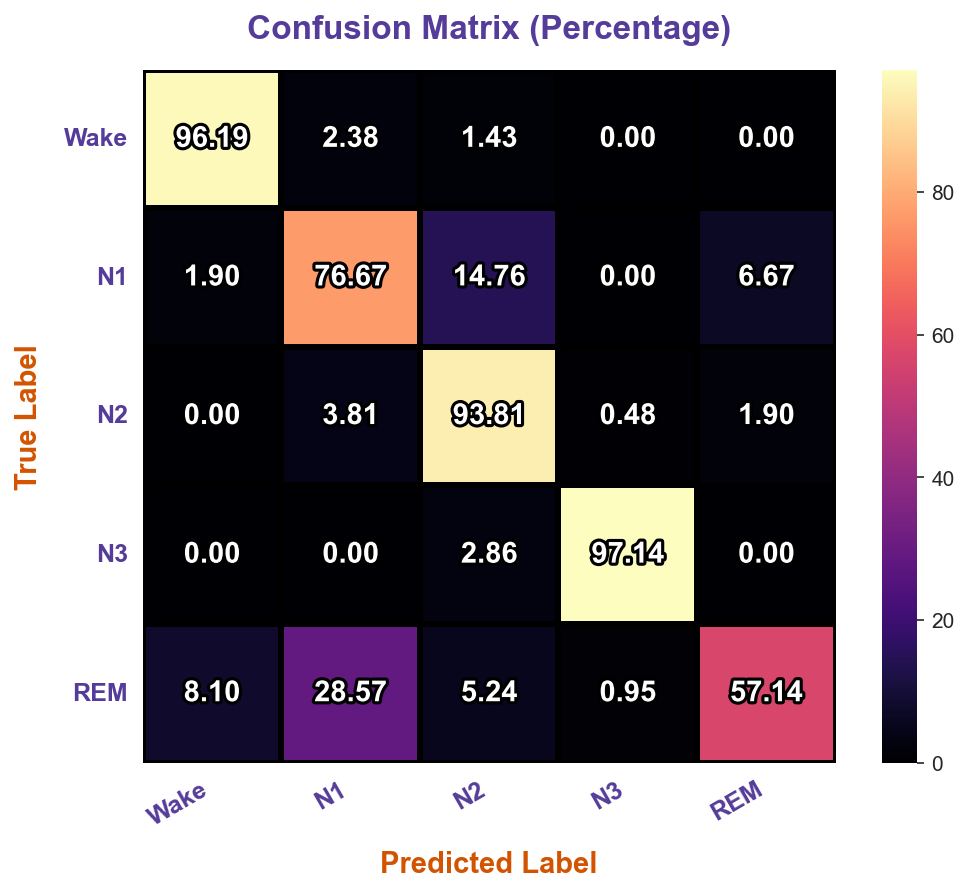
\includegraphics[width=\linewidth]{img/paper_3/confusion matrix percentatge wise}
		\caption{Confusion matrix (percentage)}
		\label{fig:confusion-matrix-percentatge-wise}
	\end{minipage}
	\hfill
	\begin{minipage}[b]{0.45\linewidth}
		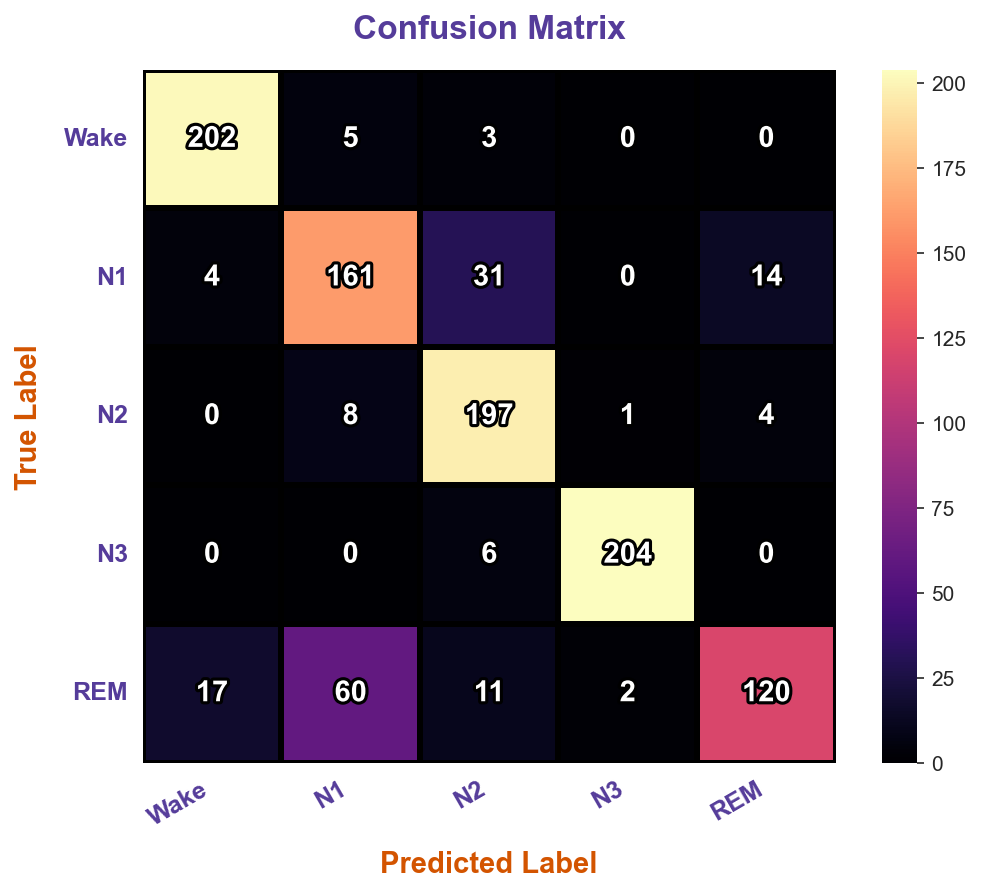
\includegraphics[width=\linewidth]{img/paper_3/confusion matrix samples}
		\caption{Confusion matrix (samples)}
		\label{fig:confusion-matrix-samples}
	\end{minipage}
\end{figure}

\begin{figure}[htbp]
	\centering
	\begin{minipage}[b]{0.45\linewidth}
		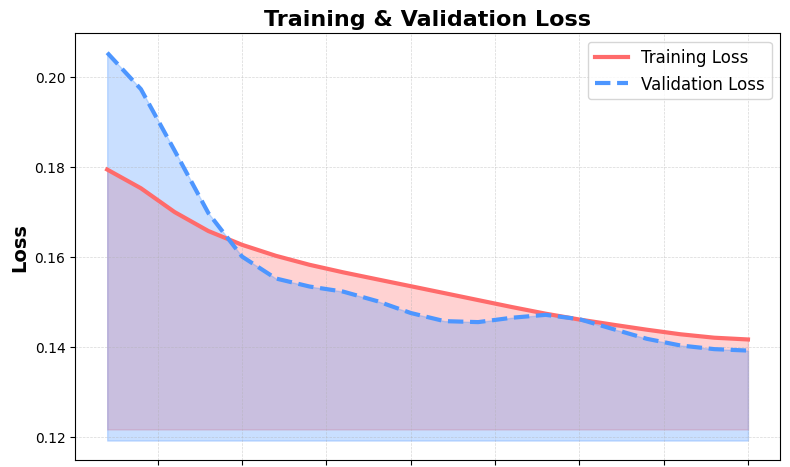
\includegraphics[width=\linewidth]{img/paper_3/loss plot}
		\caption{Loss plot}
		\label{fig:loss-plot}
	\end{minipage}
	\hfill
	\begin{minipage}[b]{0.45\linewidth}
		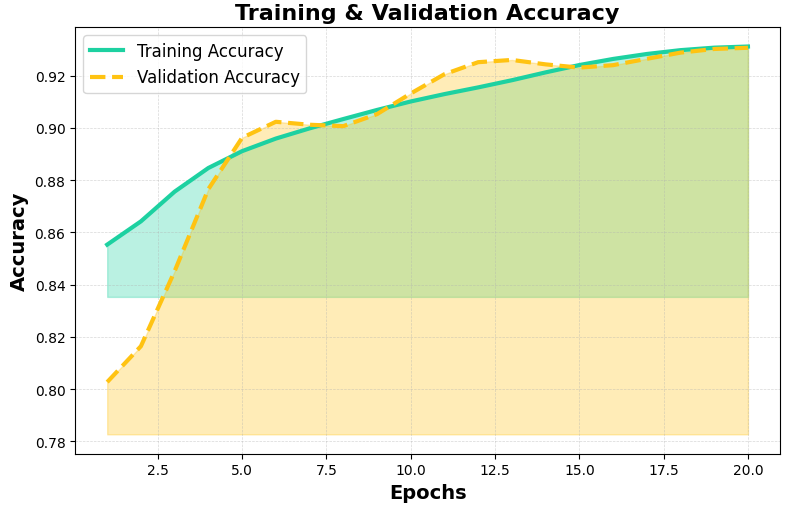
\includegraphics[width=\linewidth]{img/paper_3/accuracy plot}
		\caption{Accuracy plot}
		\label{fig:accuracy-plot}
	\end{minipage}
\end{figure}

The class weight distribution used during training is as follows: 0: 1.1923, 1: 5.8152, 2: 2.4719, 3: 4.8223, 4: 4.0506. These values reflect adjustments to counter class imbalance and ensure fairer learning across all sleep stages.

The progression of model performance across selected epochs is summarized below:
\begin{itemize}
	\item Epoch 1: Train Loss = 0.1915, Train Accuracy = 82.91\%; Validation Loss = 0.2110, Validation Accuracy = 83.84\%
	\item Epoch 2: Train Loss = 0.1695, Train Accuracy = 87.74\%; Validation Loss = 0.2168, Validation Accuracy = 69.46\%
	\item Epoch 3: Train Loss = 0.1669, Train Accuracy = 88.15\%; Validation Loss = 0.1803, Validation Accuracy = 88.39\%
	\item Epoch 4: Train Loss = 0.1659, Train Accuracy = 88.38\%; Validation Loss = 0.1534, Validation Accuracy = 91.83\%
	\item Epoch 5: Train Loss = 0.1621, Train Accuracy = 89.45\%; Validation Loss = 0.1615, Validation Accuracy = 89.11\%
	\item Epoch 10: Train Loss = 0.1533, Train Accuracy = 91.03\%; Validation Loss = 0.1471, Validation Accuracy = 91.16\%
	\item Epoch 15: Train Loss = 0.1458, Train Accuracy = 92.59\%; Validation Loss = 0.1484, Validation Accuracy = 90.98\%
	\item Epoch 20: Train Loss = 0.1413, Train Accuracy = 93.12\%; Validation Loss = 0.1390, Validation Accuracy = 93.04\%
\end{itemize}

\begin{figure}[htbp]
	\centering
	\begin{minipage}[b]{0.45\linewidth}
		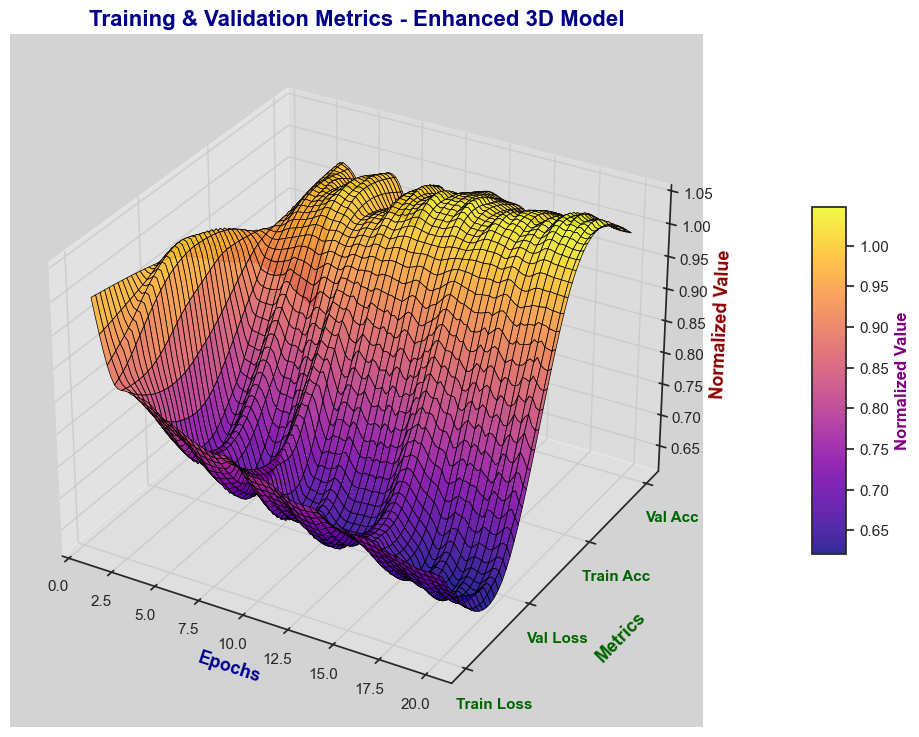
\includegraphics[width=\linewidth]{img/paper_3/3D acc loss plot}
		\caption{3D Accuracy vs. Loss}
		\label{fig:3d-acc-loss-plot}
	\end{minipage}
	\hfill
	\begin{minipage}[b]{0.45\linewidth}
		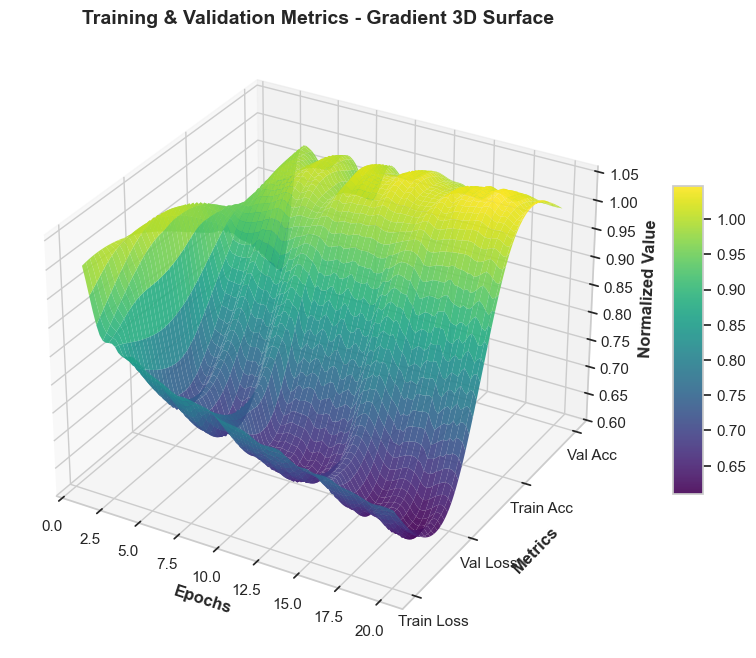
\includegraphics[width=\linewidth]{img/paper_3/3d gradient}
		\caption{3D Gradient visualization}
		\label{fig:3d-gradient}
	\end{minipage}
\end{figure}

The sample distribution plot reveals a nearly normal distribution of data across the various sleep stages, confirming a balanced dataset. For the test phase, approximately 1,050 samples were utilized, with 210 samples assigned to each class, ensuring equitable and unbiased performance evaluation.

\begin{figure}[htbp]
	\centering
	\begin{minipage}[b]{0.45\linewidth}
		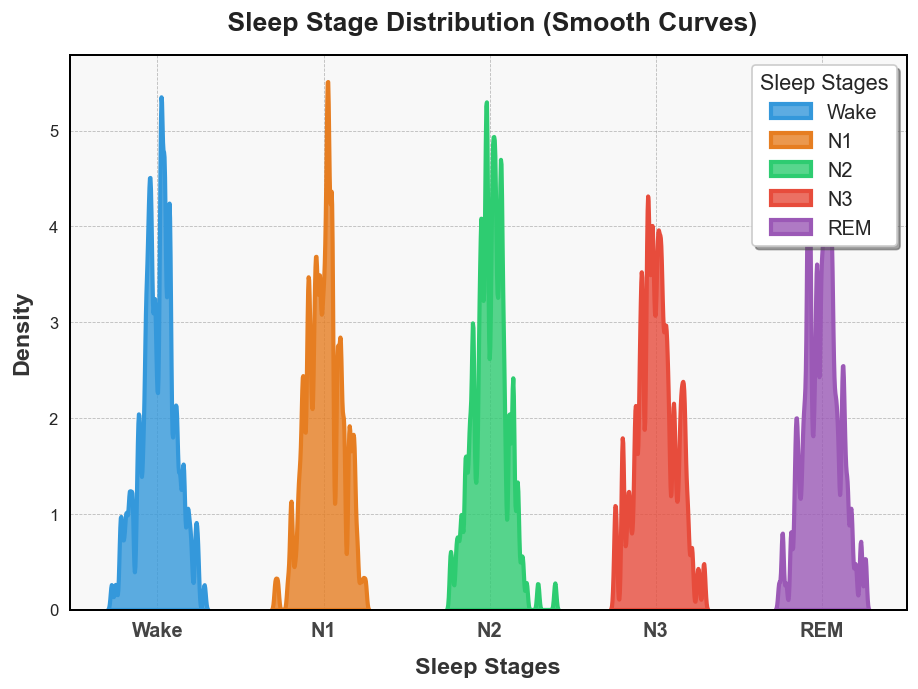
\includegraphics[width=\linewidth]{img/paper_3/sample distribution plot pdf}
		\caption{Sample distribution}
		\label{fig:sample-distribution-plot-pdf}
	\end{minipage}
	\hfill
	\begin{minipage}[b]{0.45\linewidth}
		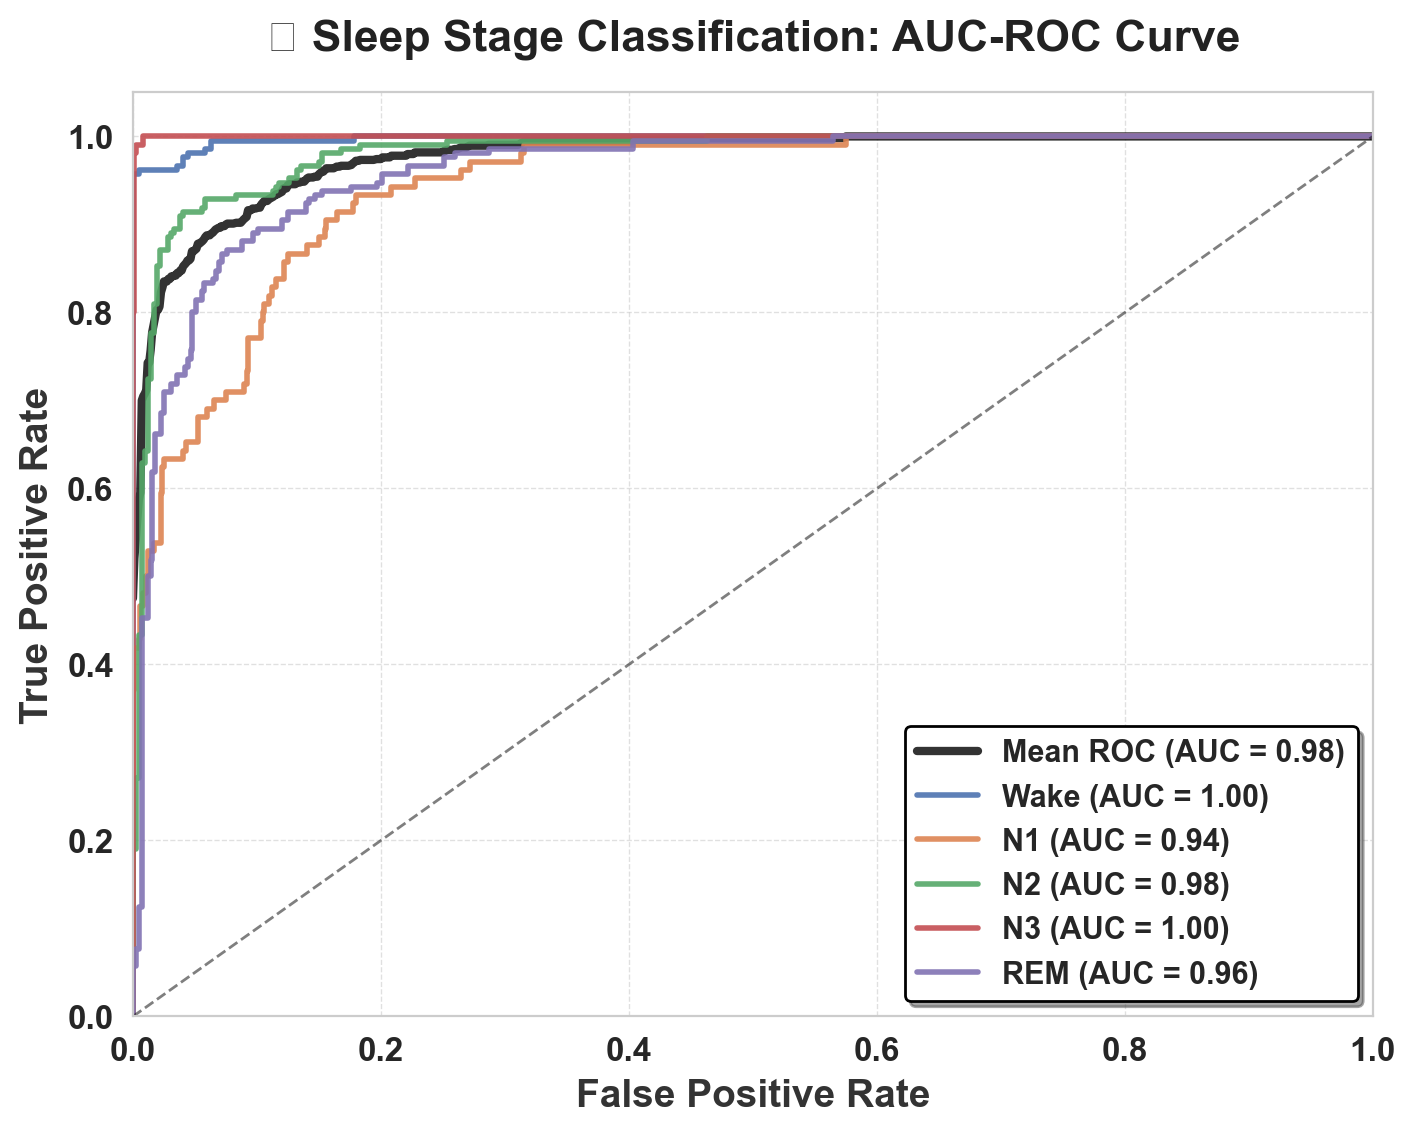
\includegraphics[width=\linewidth]{img/paper_3/auc vs roc curve}
		\caption{AUC vs. ROC Curve}
		\label{fig:auc-vs-roc-curve}
	\end{minipage}
\end{figure}

\begin{figure}[htbp]
	\centering
	\begin{minipage}[b]{0.31\linewidth}
		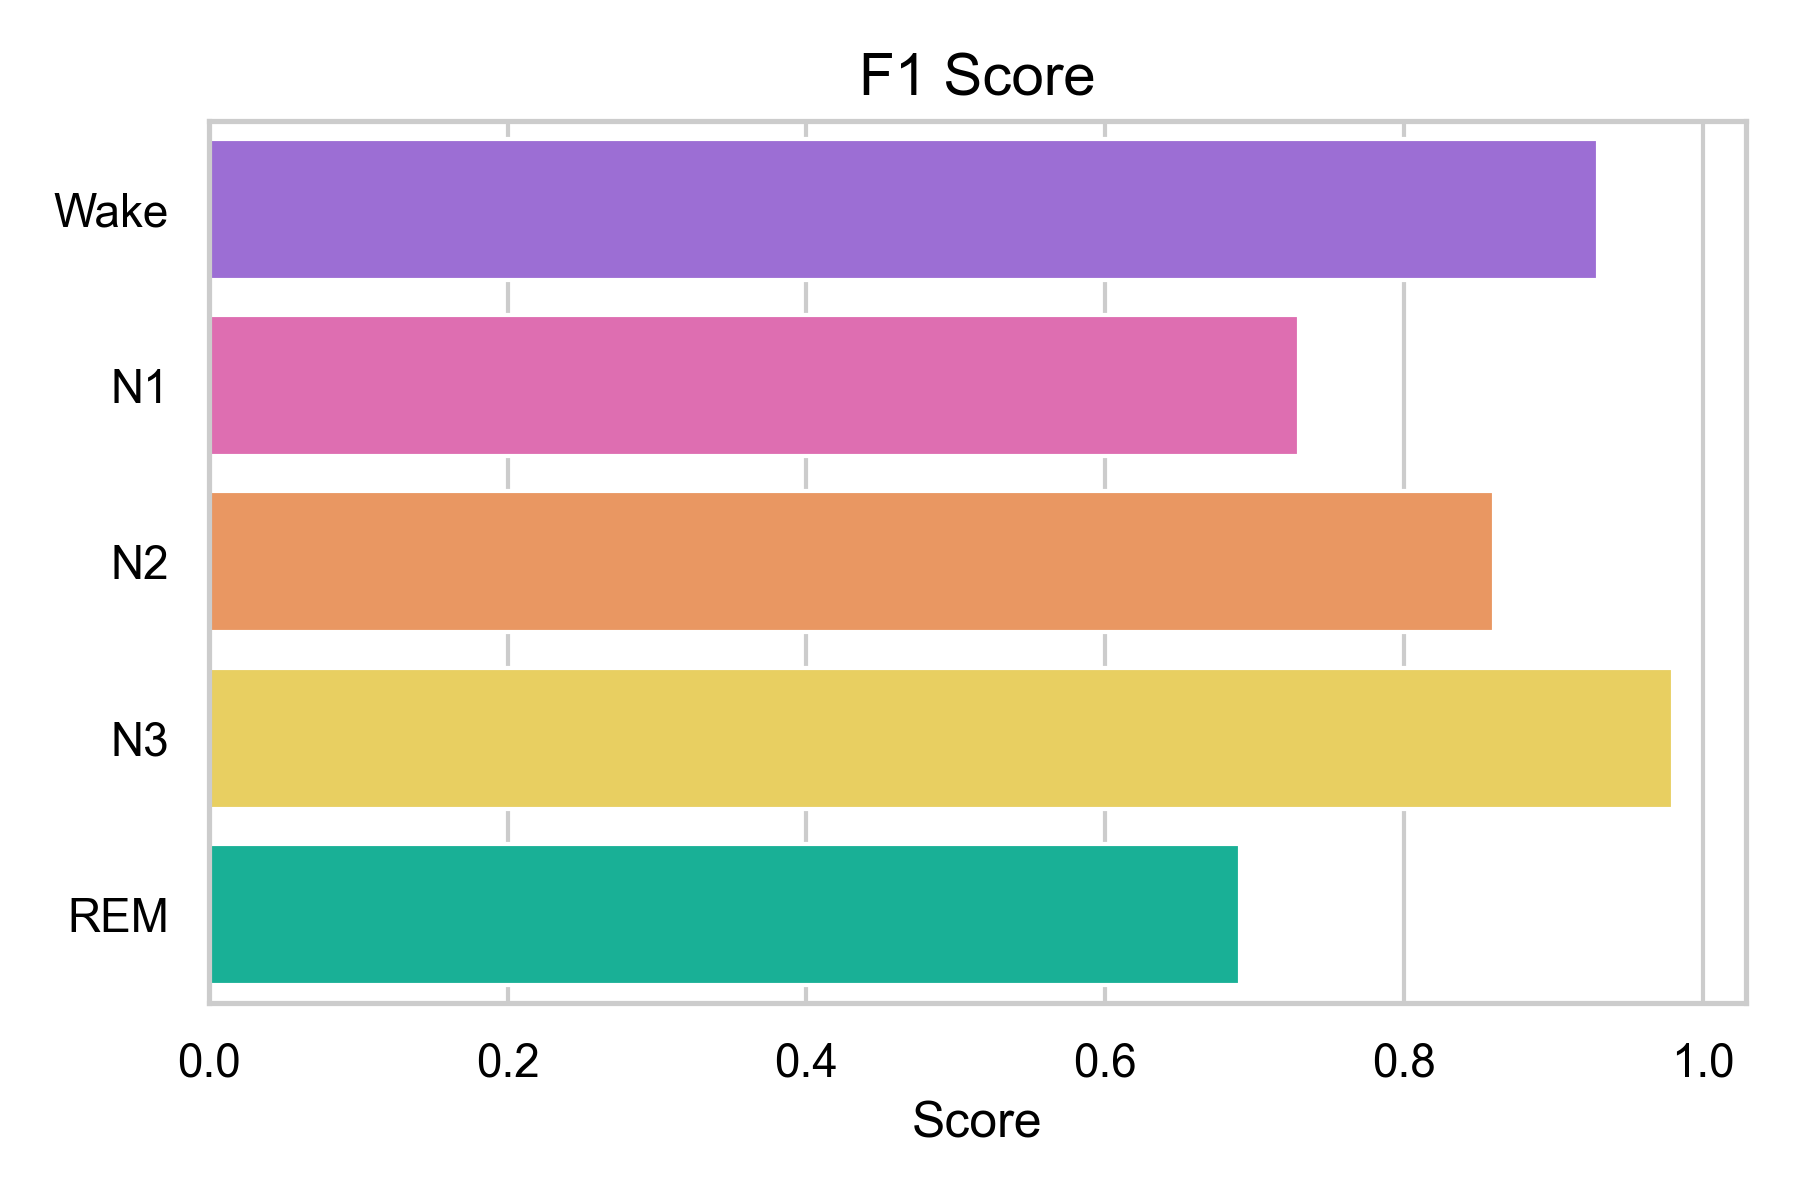
\includegraphics[width=\linewidth]{img/paper_3/f1_score_plot}
		\caption{F1 Score}
		\label{fig:f1scoreplot}
	\end{minipage}
	\hfill
	\begin{minipage}[b]{0.31\linewidth}
		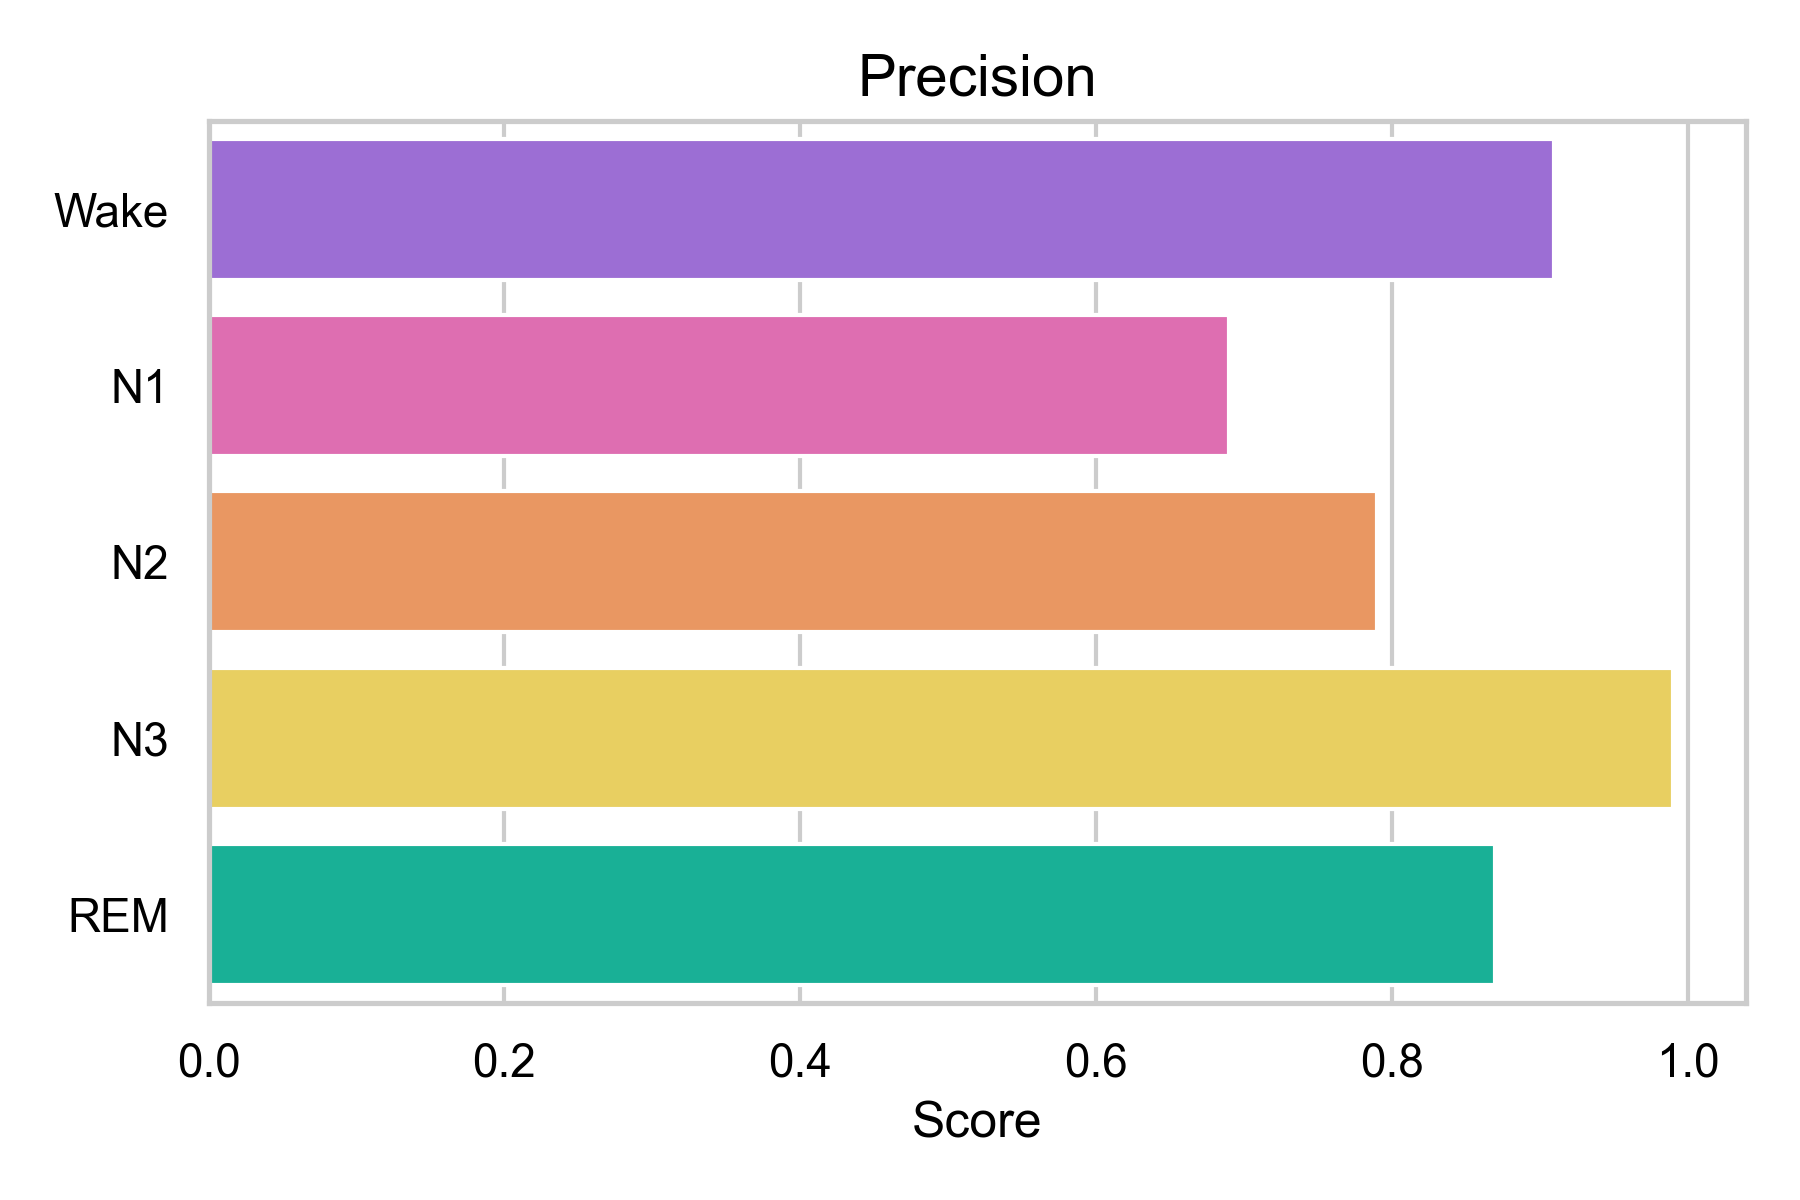
\includegraphics[width=\linewidth]{img/paper_3/precision_plot}
		\caption{Precision}
		\label{fig:precisionplot}
	\end{minipage}
	\hfill
	\begin{minipage}[b]{0.31\linewidth}
		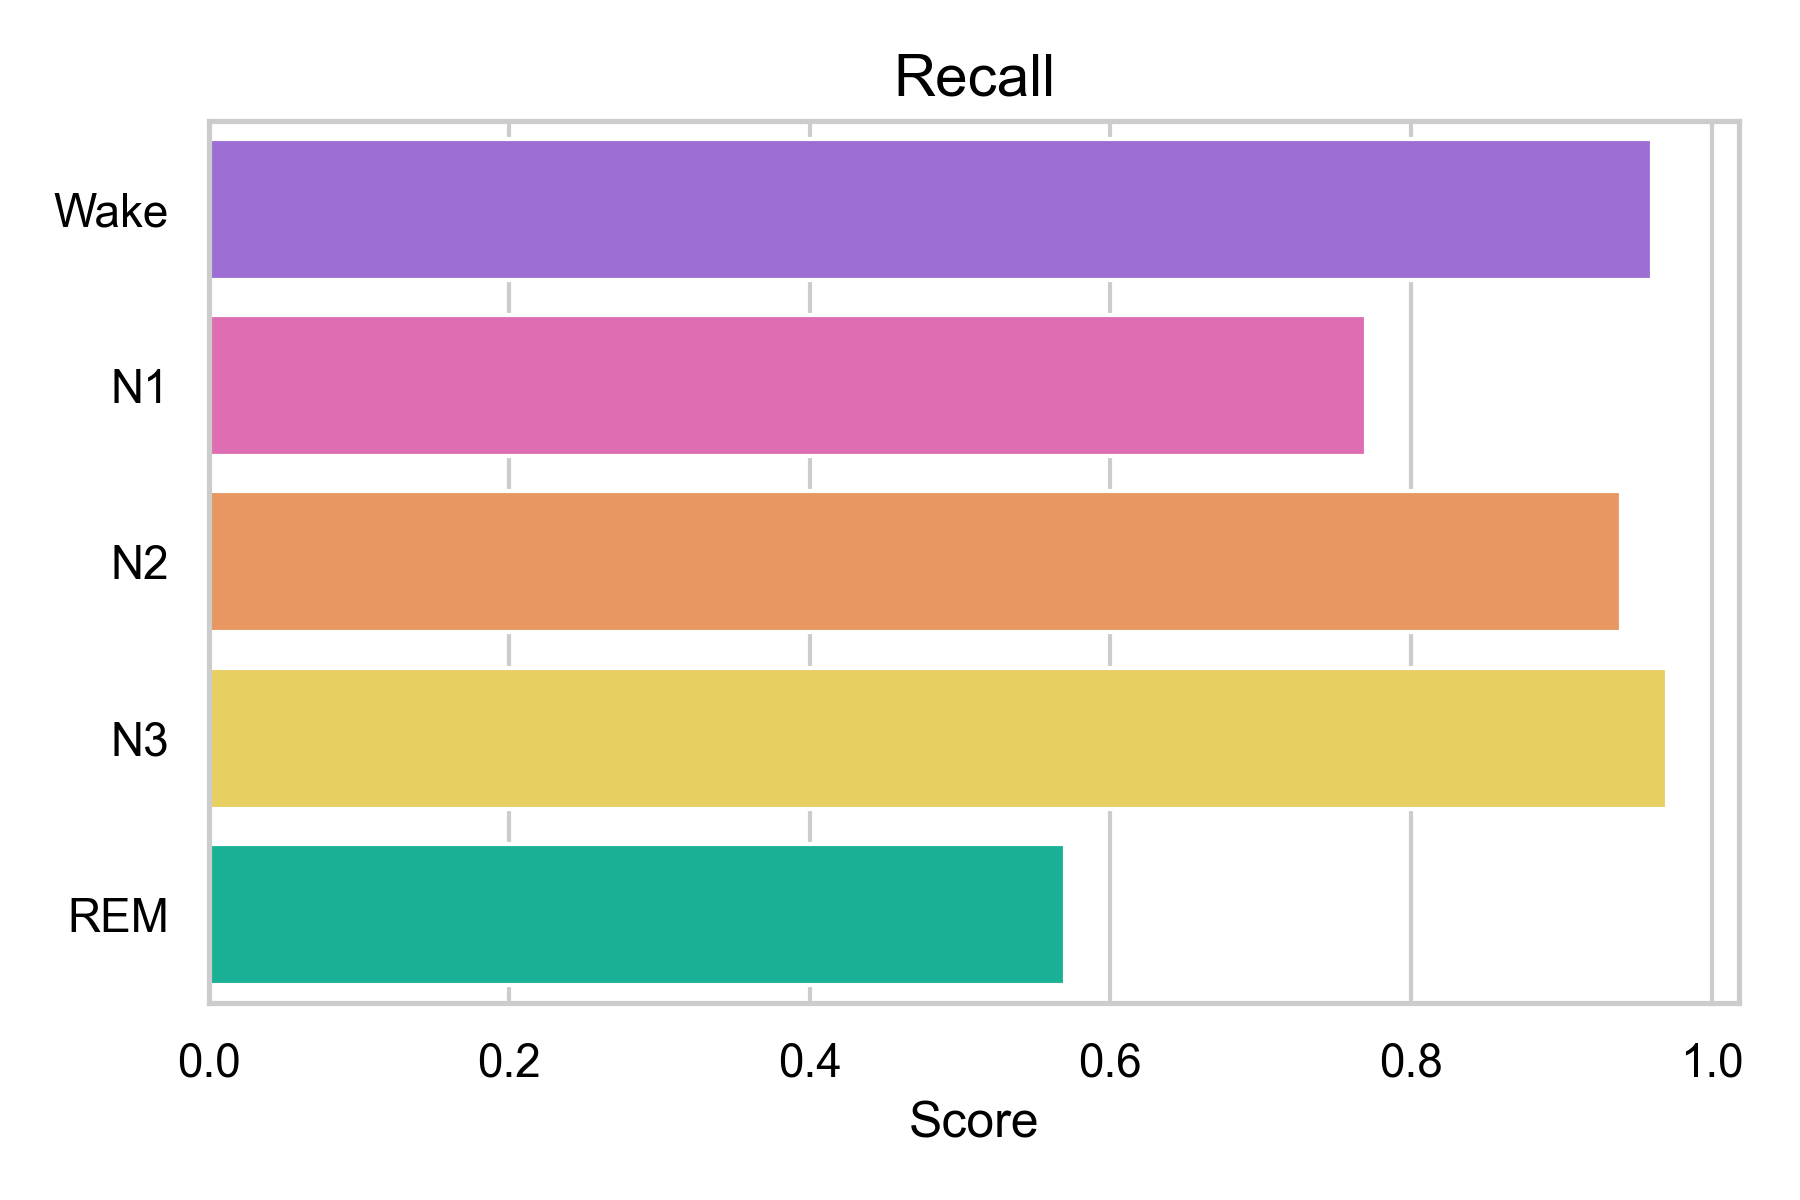
\includegraphics[width=\linewidth]{img/paper_3/recall_plot}
		\caption{Recall}
		\label{fig:recallplot}
	\end{minipage}
\end{figure}



















\subsection{XAI Visualization with Heatmap and Plots}

\begin{figure}[H]
	\centering
	\begin{minipage}[b]{0.45\linewidth}
		\includegraphics[width=\linewidth]{"img/paper_3/stage n1"}
		\caption{Stage N1}
		\label{fig:stage-n1}
	\end{minipage}
	\hfill
	\begin{minipage}[b]{0.45\linewidth}
		\includegraphics[width=\linewidth]{"img/paper_3/stage n2"}
		\caption{Stage N2}
		\label{fig:stage-n2}
	\end{minipage}
\end{figure}

\begin{figure}[htbp]
	\centering
	\begin{minipage}[b]{0.45\linewidth}
		\includegraphics[width=\linewidth]{"img/paper_3/stage n3"}
		\caption{Stage N3}
		\label{fig:stage-n3}
	\end{minipage}
	\hfill
	\begin{minipage}[b]{0.45\linewidth}
		\includegraphics[width=\linewidth]{"img/paper_3/stage rem"}
		\caption{Stage REM}
		\label{fig:stage-rem}
	\end{minipage}
\end{figure}

\begin{figure}[htbp]
	\centering
	\begin{minipage}[b]{0.45\linewidth}
		\includegraphics[width=\linewidth]{"img/paper_3/stage wake"}
		\caption{Stage Wake}
		\label{fig:stage-wake}
	\end{minipage}
	\hfill
	\begin{minipage}[b]{0.45\linewidth}
		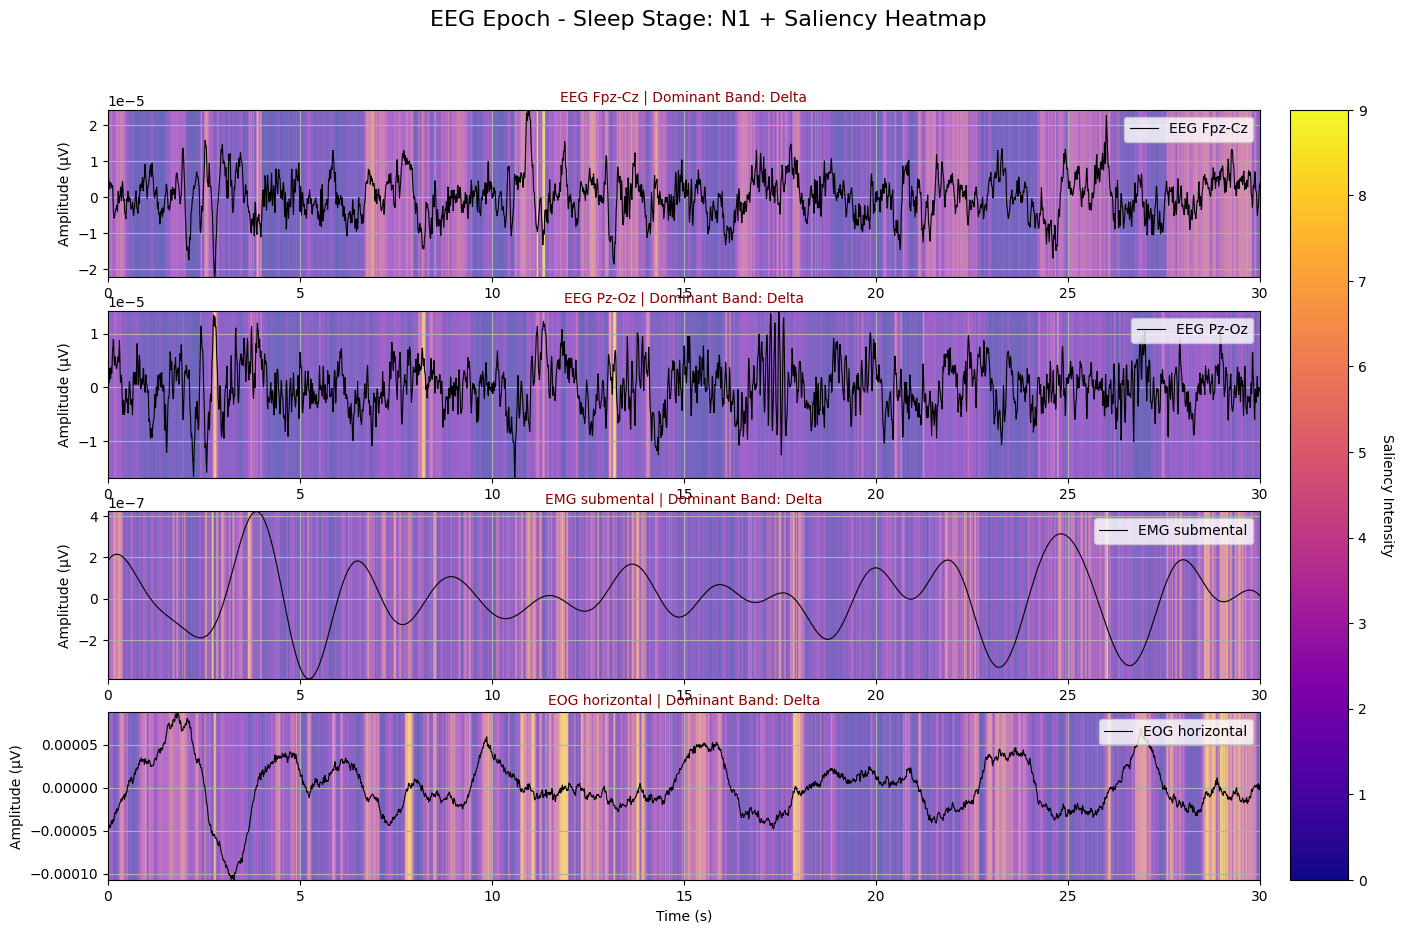
\includegraphics[width=\linewidth]{img/paper_3/XAI4}
		\caption{XAI Visualization}
		\label{fig:xai4}
	\end{minipage}
\end{figure}










































\subsection{Time Complexity Analysis}

\begin{figure}[H]
	\centering
	\begin{minipage}[b]{0.40\linewidth}
		\centering
		\includegraphics[width=\linewidth]{img/paper_3/preprocessing_on³}
		\caption{Preprocessing (\(O(MN^3 + KEN + MN)\))}
		\label{fig:preprocessingon3}
	\end{minipage}
	\hfill
	\begin{minipage}[b]{0.40\linewidth}
		\centering
		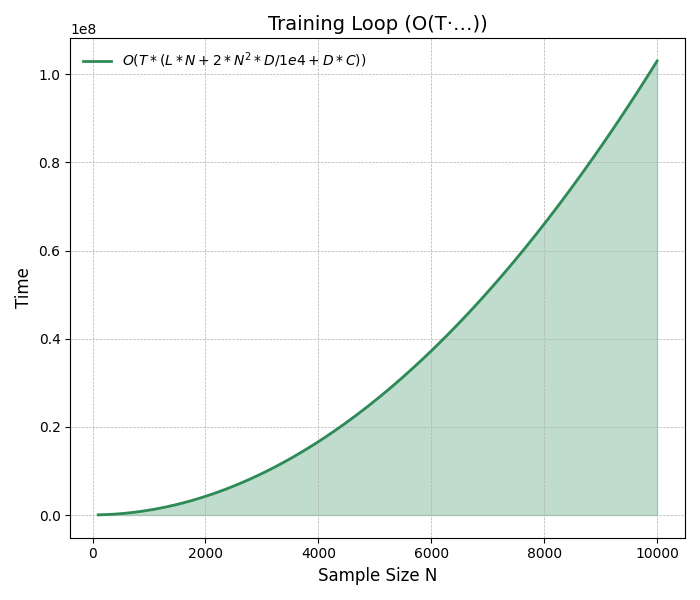
\includegraphics[width=\linewidth]{img/paper_3/training_loop_ot·…}
		\caption{Training Loop (\(O(T(LN + 2N^2D/10^4 + DC))\))}
		\label{fig:trainingloopot}
	\end{minipage}
\end{figure}

\noindent Preprocessing: \(O(MN^3 + KEN + MN)\) \\
Training Loop: \(O(T(LN + 2N^2D/10^4 + DC))\)

\begin{figure}[H]
	\centering
	\begin{minipage}[b]{0.40\linewidth}
		\centering
		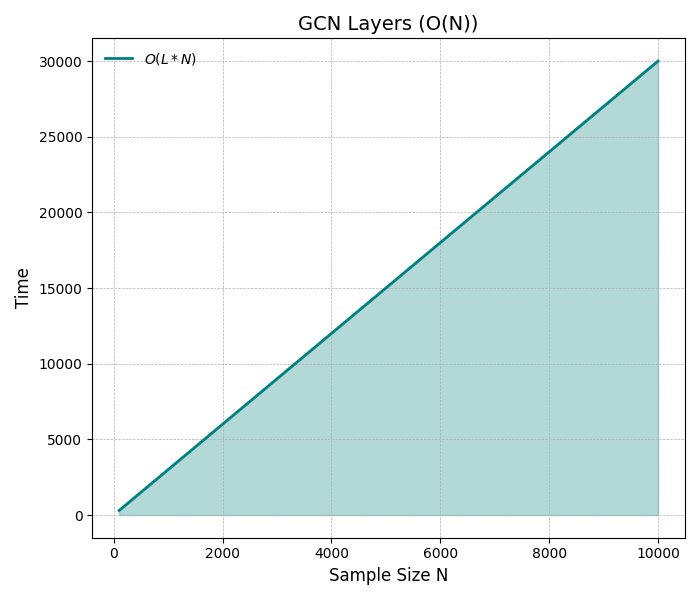
\includegraphics[width=\linewidth]{img/paper_3/gcn_layers_on}
		\caption{GCN Layers (\(O(LN)\))}
		\label{fig:gcnlayerson}
	\end{minipage}
	\hfill
	\begin{minipage}[b]{0.40\linewidth}
		\centering
		\includegraphics[width=\linewidth]{img/paper_3/transformer_encoder_on²}
		\caption{Transformer Encoder (\(O(N^2D)\))}
		\label{fig:transformerencoderon2}
	\end{minipage}
\end{figure}

\noindent GCN Layers: \(O(LN)\) \\
Transformer Encoder: \(O(N^2D)\)

\begin{figure}[H]
	\centering
	\begin{minipage}[b]{0.40\linewidth}
		\centering
		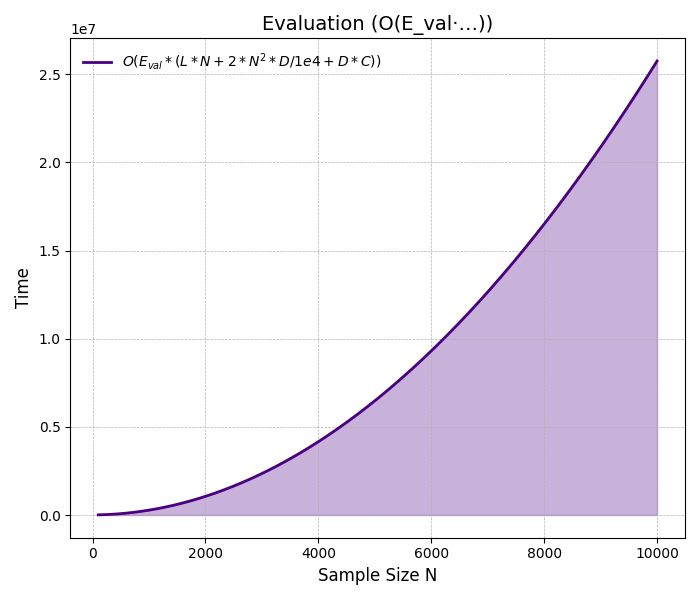
\includegraphics[width=\linewidth]{img/paper_3/evaluation_oe_val·…}
		\caption{Evaluation Loop (\(O(E_{\text{val}}(LN + 2N^2D/10^4 + DC))\))}
		\label{fig:evaluationoeval}
	\end{minipage}
	\hfill
	\begin{minipage}[b]{0.40\linewidth}
		\centering
		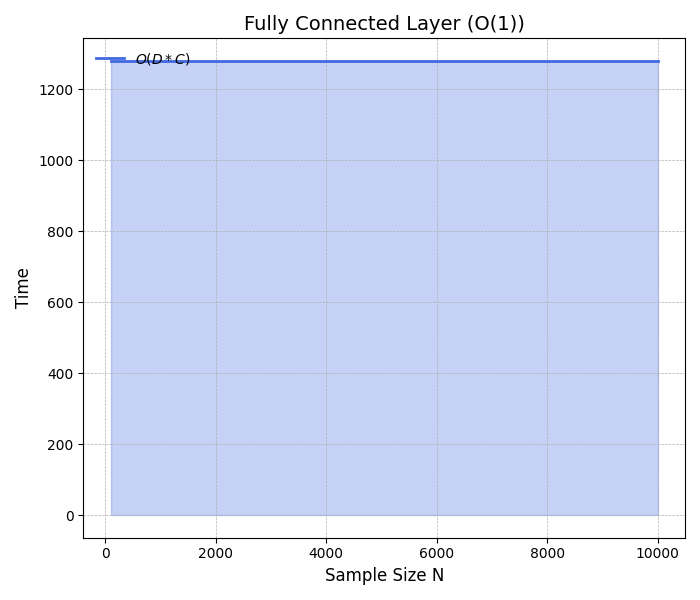
\includegraphics[width=\linewidth]{img/paper_3/fully_connected_layer_o1}
		\caption{Fully Connected Layer (\(O(DC)\))}
		\label{fig:fullyconnectedlayero1}
	\end{minipage}
\end{figure}

\noindent Evaluation Loop: \(O(E_{\text{val}}(LN + 2N^2D/10^4 + DC))\) \\
Fully Connected Layer: \(O(DC)\)
